\documentclass[aspectratio=169,11pt]{beamer}
\usepackage[T1]{fontenc}
\usepackage{lmodern}
\usepackage{booktabs}
\usepackage{tikz}
\usetikzlibrary{arrows.meta,positioning}

% A plain look: sans-serif, no navigation symbols, one accent colour.
\usetheme{default}
\usefonttheme{professionalfonts}
\renewcommand{\familydefault}{\sfdefault}
\definecolor{accent}{HTML}{1F5FA8}
\setbeamercolor{structure}{fg=accent}
\setbeamercolor{frametitle}{fg=accent}
\setbeamertemplate{navigation symbols}{}
\setbeamertemplate{footline}{\hfill\insertframenumber/\inserttotalframenumber\hspace{1em}\vspace{0.5em}}
\setbeamertemplate{itemize items}[circle]

\title{Title of the Talk}
\subtitle{One line that says what the audience will take home}
\author{Your Name}
\institute{Institution}
\date{Conference or Seminar, \today}

\begin{document}

\begin{frame}[plain]
  \titlepage
\end{frame}

\begin{frame}{Outline}
  \tableofcontents
\end{frame}

\section{Motivation}
\begin{frame}{The problem in one slide}
  \begin{itemize}
    \item One idea per slide; say the rest aloud.
    \item Use at most four bullets of a line each.
    \item End the slide on its message, not on a list.
  \end{itemize}
\end{frame}

\section{Approach}
\begin{frame}{Two columns: text and a picture}
  \begin{columns}[T]
    \begin{column}{0.5\textwidth}
      A diagram explains faster than prose:
      \begin{itemize}
        \item data goes in
        \item the model transforms it
        \item results come out
      \end{itemize}
    \end{column}
    \begin{column}{0.5\textwidth}
      \centering
      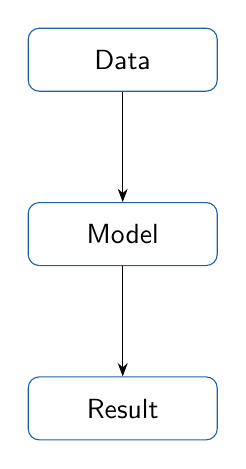
\begin{tikzpicture}[node distance=1.4cm, >=Stealth,
          box/.style={draw=accent, rounded corners, minimum width=2.4cm, minimum height=0.8cm}]
        \node[box] (in) {Data};
        \node[box, below=of in] (m) {Model};
        \node[box, below=of m] (out) {Result};
        \draw[->] (in) -- (m);
        \draw[->] (m) -- (out);
      \end{tikzpicture}
    \end{column}
  \end{columns}
\end{frame}

\begin{frame}{Blocks for definitions and results}
  \begin{block}{Definition}
    A highlighted statement the audience should remember.
  \end{block}
  \begin{alertblock}{Caveat}
    Something that does not work yet, flagged honestly.
  \end{alertblock}
  \begin{exampleblock}{Example}
    $e^{i\pi} + 1 = 0$
  \end{exampleblock}
\end{frame}

\section{Results}
\begin{frame}{Results}
  \centering
  \begin{tabular}{lcc}
    \toprule
    Method & Error & Time \\
    \midrule
    Baseline & 12.4\% & 38 ms \\
    Ours & \textbf{8.1\%} & 41 ms \\
    \bottomrule
  \end{tabular}
\end{frame}

\begin{frame}{Take-home messages}
  \begin{enumerate}
    \item First finding.
    \item Second finding.
    \item What to do next.
  \end{enumerate}
  \vfill\centering\Large Thank you. Questions?
\end{frame}

\begin{frame}{Backup: extra details}
  Keep extra slides for the question round after the closing slide. Putting
  \texttt{\textbackslash appendix} before them hides them from the slide numbering.
\end{frame}

\end{document}
